\chapter{Theoretische Grundlagen}
\label{chap:two}
\section{Bibliothek und Statistik}
\label{chap:two_one}
Warum ist Messbarkeit von bibliothekarischen Daten wichtig?\\
Erhebung von qualitativen und quantitativen Daten Bsp.:\\

Konzentration auf quantitative Daten wie ...\\
Welche quantitativen Daten werden in Bibliotheken erhoben\\
...\\
Begriffe wie Mittelallokation\\
Bestandsmanagement\\
Nutzungsanalyse\\
Counter-Statistiken \& Standards
Bestandsanalyse -und Evaluierung\\
Was können statistische Daten in Bibliotheken aussagen?\\
Welchen Impact für Budgetplanung können statistische Daten haben?\\
Counter5-Statistiken


\section{Datenvisualisierung}
Mit den Siegeszug des Computers in den 1980/90er Jahren sind \dots\\



Was ist unter Datenvisualisierung zu verstehen?\\
leicht verschiedene Begriffsdefinitionen
Vielzahl von Begriffen\\ Oberbegriff für Informationsvisualisierung / Scientific Visualization\\
Abgrenzung zu Infographics\\
Zu welchem Zweck\\
Wie Datenvisualisierungen gestaltet werden sollen - simpel\\
Grundlage - Daten 

Warum Datenvisualisierung wichtig ist?\\
Welche Datenvisualisierungen gibt es?\\
Was erzählen Datenvisualisierungen mehr als Zahlenkolonnen?\\
Wo kommen Daternvisualisierungen zum Einsatz?\\
Was ist unter Datenvisualisierungstechniken zu verstehen?\\
Wo kommen Datenvisualisierungstechniken zum Einsatz?


\begin{figure}[ht]
    \centering
        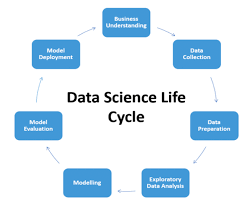
\includegraphics[width=8cm]{ds_cycle}
        \caption{Data Science Cycle}
        \label{fig:data science}
\end{figure}




\section{Business-Intelligence-Systeme}

Was sind Business-Intelligence-Löungen?\\
Wo kommen Buisiness-Intelligence-Lösungen zum Einsatz zum Einsatz?
